% Solução após Esau-Williams: s-tree {1,2} e s-tree {3,4}
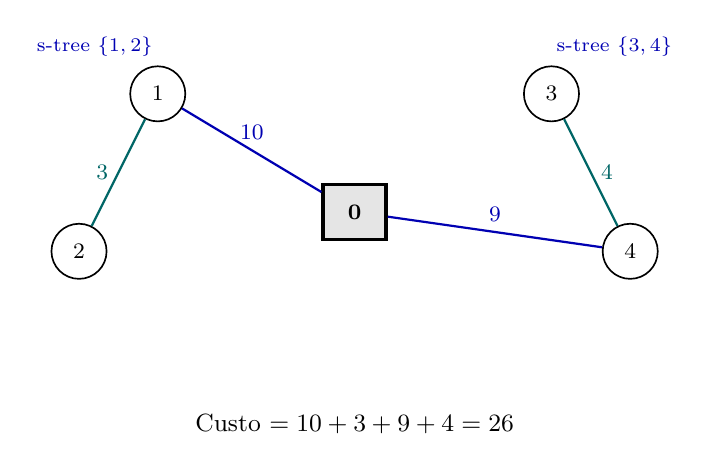
\begin{tikzpicture}
\tikzset{
    >=stealth,
    gate/.style={-, thick, blue!70!black},
    interna/.style={-, thick, teal!80!black},
    vertice/.style={circle, semithick, draw=black, inner sep=0pt, minimum size=0.7cm},
    raiz/.style={rectangle, very thick, draw=black, fill=gray!20,
                 minimum width=0.8cm, minimum height=0.7cm}
}
\node[raiz]    (v0) at (2.5, 2)   {\footnotesize \textbf{0}};
\node[vertice] (v1) at (0,   3.5) {\footnotesize 1};
\node[vertice] (v2) at (-1,  1.5) {\footnotesize 2};
\node[vertice] (v3) at (5,   3.5) {\footnotesize 3};
\node[vertice] (v4) at (6,   1.5) {\footnotesize 4};
% Gates (ligações de cada s-tree à raiz)
\draw[gate] (v0) -- node[above, font=\footnotesize] {10} (v1);
\draw[gate] (v0) -- node[above, font=\footnotesize] {9}  (v4);
% Arestas internas (economias realizadas)
\draw[interna] (v1) -- node[left,  font=\footnotesize] {3} (v2);
\draw[interna] (v4) -- node[right, font=\footnotesize] {4} (v3);
% Rótulos das s-trees
\node[font=\scriptsize, color=blue!70!black] at (-0.8, 4.1) {s-tree $\{1,2\}$};
\node[font=\scriptsize, color=blue!70!black] at (5.8,  4.1) {s-tree $\{3,4\}$};
\node[font=\small, align=center] at (2.5,-0.7) {Custo $= 10+3+9+4 = 26$};
\end{tikzpicture}
